% !TEX program = lualatex
\documentclass[
    bibliography=totoc,
    listof=totoc,
    listof=entryprefix,
    toc=sectionentrywithdots
]{scrreprt}
\usepackage[english]{babel}
\usepackage{lmodern,lipsum,microtype}
\usepackage[UPC]{tensygrid}
\geometry{
  paper=a4paper,
  left=25mm,
  right=25mm,
  top=25mm,
  bottom=25mm,
  bindingoffset=0mm,
  marginparwidth=0pt,
  marginparsep=0pt,
  includeheadfoot
}
\usepackage{tikz}
\usetikzlibrary{positioning}
\usepackage{mathtools}
\usepackage{ieeetrantools}
\usepackage{siunitx}
\usepackage{bm}
\usepackage{circuitikz}
\usepackage{amsmath}
\usepackage{rotating}
\usepackage{float}
\usepackage{amssymb}
\usepackage{xcolor}
%\usepackage[sections]{placeins}
\usepackage{booktabs}
\usepackage{enumitem}

\newcommand{\ra}[1]{\renewcommand{\arraystretch}{#1}}

\usepackage[backend=biber, sorting=none]{biblatex}
\addbibresource{ref.bib}  % Adjust to your .bib file name

\author{Alexandre~Gràcia~Calvo\\Carlos~Herrera~Vázquez\\Dr.~Eduardo~Prieto~Araujo}
\title{TenSyGrid Toolbox: Use cases identification and description }
\setkomavar{docname}{Deliverable Report}
\subject{Deliverable Report}
\setkomavar{docnumber}{D4.1}
\setkomavar{projectnumber}{CETP-FP-2023-00138}
\setkomavar{workpackage}{WP 4}
\setkomavar{version}{v1.1.0}
\setkomavar{callman}{CETPartnership}
\setkomavar{toname}{Universitat Politècnica de Catalunya}
\setkomavar{fromphone}{30/11/2026}
\setkomavar{toaddress}{%
CETPartnership \\
  Call Management}
\setkomavar{fromname}{Alexandre~Gràcia~Calvo\\Carlos~Herrera~Vázquez\\Dr.~Eduardo~Prieto~Araujo}
\setkomavar{yourref}{Universitat Politècnica de Catalunya}
\setkomavar{director}{Dr.~Eduardo~Prieto~Araujo}
\setkomavar{projectcoordinator}{Dr.~Carlos~Cateriano~Yáñez}
\setkomavar{classification}{Public} % Confidential or Public
\colorlet{classificationcolor}{tgred} % tgred CO tglime PU
\setkomavar{contributions}{}
\subtitle{Project: Tensors for System Analysis of\\ Converter-dominated Power Grids}
\date{31 October 2026}
\tgsigsetup{
  fromname         = {Alexandre~Gràcia~Calvo\\Carlos~Herrera~Vázquez},
  fromfunction     = {Phd Student\\Phd Student},
  headname         = {Dr.~Carlos~Cateriano~Yáñez},
  headfunction     = {Project Coordinator},
  reviewername     = {Dr.~John Licari},
  reviewerfunction = {Principal Investigator at UM},
}

\BeforeStartingTOC[lof]{\def\autodot{:}}
\BeforeStartingTOC[lot]{\def\autodot{:}}

\begin{document}
{\raggedright
\maketitle}
\section*{Acknowledgement}
\insertack
\vspace*{2ex}
\newline
{\center
\insertcallorg}
\newline
{\center
\insertagencies}
\clearpage
\section*{About TenSyGrid}
\insertabout
\vspace*{8ex}
\newline
\textbf{Project coordinator:}
{\center
\insertcoord}
\vspace*{2ex}
\newline
\textbf{Consortium:}
{\center
\insertconsortium}
\newline
\clearpage

\section*{Summary}
This deliverable identifies and describes the use cases that the TenSyGrid Toolbox must support to serve network operators in assessing the small-signal stability of converter-dominated power grids. Fourteen use cases are catalogued and described, organised into two groups: six use cases already prototyped in an initial web-based Stability Monitor, and eight additional use cases proposed for discussion with operators during a dedicated workshop.

The implemented use cases cover the core stability-analysis workflow: launching a small-signal eigenvalue computation, inspecting the system status via a dashboard, exploring the eigenvalue spectrum, diagnosing critical oscillation modes through participation factors, verifying bus voltage profiles, and performing N-1 contingency analysis with some recommendations.



\tableofcontents
\listoffigures
\listoftables
\clearpage

\chapter{Introduction}
The transition towards converter-dominated power systems, driven by the massive integration of renewable energy sources, is fundamentally altering the dynamic behaviour of electrical grids. As synchronous generation is progressively displaced by inverter-based resources, new stability challenges emerge: reduced system inertia, faster electromagnetic transients, and complex interactions between converter controls and the network. In this context, transmission system operators require tools that can assess stability rapidly, reliably, and under a wide range of operating scenarios.

The European project \textit{TenSyGrid} addresses this need by developing a toolbox for direct stability assessment based on a tensor (multilinear) reformulation of power system component models. By expressing the nonlinear dynamics of generators, converters, lines, loads, and transformers in a multilinear form, the toolbox enables efficient computation of the system's state matrix and its eigenvalues, which are the fundamental indicators of small-signal stability. The toolbox is designed to be compatible with existing commercial software packages, facilitating its integration into current operator workflows.

This deliverable (D4.1) constitutes the first step in Work Package~4 (\textit{TenSyGrid Toolbox Development}). Its objective is to identify, describe, and catalogue the use cases that the toolbox must support, taking the network operator as the primary user. The use cases are derived from three complementary sources:

\begin{enumerate}
  \item The TenSyGrid project objectives, as defined in the CETPartnership proposal.
  \item An initial web-based \textit{Stability Monitor} prototype that implements core stability-analysis workflows.
  \item An anticipated operator-needs analysis, to be validated during a dedicated workshop with grid operators.
\end{enumerate}

The document is structured as follows. Chapter~2 describes the methodological approach, the evolution of the software architecture towards a native open-source Python framework, and the insights gathered from operator interviews. Chapter~3 presents the use case inventory, organised into implemented and proposed use cases, and outlines the organization of the toolbox interface. Each use case is described in terms of its actor, objective, theoretical basis, interaction flow, and expected outcome. The chapter also documents use cases that were considered but discarded or deferred, together with the rationale for their exclusion. Chapter~4 concludes the deliverable and outlines the next steps towards the operator workshop and the subsequent development cycle.

The intended audience for this deliverable includes the TenSyGrid consortium partners, the CETPartnership review bodies, and --- after the operator workshop --- the network operators who will ultimately use and benefit from the toolbox.


\chapter{Use Cases}
\section{Use case inventory}

Table~\ref{tab:uc-inventory} provides a summary of all identified use cases, grouped by their current implementation status. The first five have been prototyped in the Stability Monitor GUI; the remaining nine are candidates to be presented and discussed with network operators.

\begin{table}[H]
  \centering
  \caption{Use case inventory for the TenSyGrid Toolbox.}
  \label{tab:uc-inventory}
  \begin{tabular}{lp{0.30\textwidth}p{0.15\textwidth}p{0.40\textwidth}}
    \toprule
    \textbf{ID} & \textbf{Name}                                  & \textbf{Status} & \textbf{Objective}                                                                     \\
    \midrule
    UC-01       & Run Small-Signal Stability Simulation          & Implemented     & Execute a stability computation on a grid model                                        \\
    UC-02       & System Status Dashboard \& Eigenvalue Spectrum & Implemented     & Obtain an at-a-glance stability classification and explore the eigenvalue distribution \\
    UC-03       & Critical Mode Diagnosis                        & Implemented     & Identify low-damped modes and their physical origin                                    \\
    UC-04       & Bus Voltage Assessment                         & Implemented     & Verify voltage profile from the power-flow solution                                    \\
    UC-05       & N-1 Contingency Analysis                       & Implemented     & Evaluate stability impact of single-element outages                                    \\
    \midrule
    UC-06       & Operating Scenario Comparison                  & Proposed        & Compare stability between two grid snapshots                                           \\
    UC-07       & Critical Device List                           & Proposed        & Rank devices by their participation in the critical modes                              \\
    UC-08       & Stability Trend Analysis                       & Proposed        & Track stability evolution across multiple operating points                             \\
    UC-09       & Critical Element Ranking                       & Proposed        & Rank elements by their contribution to stability degradation                           \\
    UC-10       & Damping Controller Placement Guidance          & Proposed        & Suggest candidate locations for PSS or FACTS devices                                   \\
    UC-11       & Renewable Scenario Assessment                  & Proposed        & Evaluate stability at different renewable penetration levels                           \\
    UC-12       & Automated Stability Report Generation          & Proposed        & Produce a standardised stability report for stakeholders                               \\
    UC-13       & Centre Manifold Analysis                       & Proposed        & Characterise the dynamics behind zero eigenvalues                                      \\
    UC-14       & Basin of Attraction Estimation                 & Proposed        & Quantify security margins against specified disturbances                               \\
    %   UC-15       & <name>                                & Proposed        & <objective>                                                  \\
    \bottomrule
  \end{tabular}
\end{table}

\section{Implemented use cases}

The following five use cases have been prototyped in the TenSyGrid Stability Monitor, a web-based graphical interface that communicates with the native Python TenSyGrid calculation engine (the ported MTI implementation integrated within VeraGrid), running on a dedicated backend server. 

% ---------------------------------------------------------------------------
\subsection{UC-01: Assessment of small-signal stability under given operating conditions}
% ---------------------------------------------------------------------------

\begin{description}
  \item[Actor.] Network operator or planning engineer.
  \item[Objective.] Load a grid model and compute its small-signal stability properties using the tensor-based multilinear formulation.
  \item[Preconditions.]
        \begin{itemize}[before=\leavevmode, leftmargin=*]
          \item The TenSyGrid engine backend is running and accessible via a web browser.
          \item At least one valid grid model is available. It may be supplied as a native \texttt{.veragrid} file, through any file format supported by VeraGrid's import layer, through the IPSA adapter from an external tool, or through a configured API endpoint.
          \item External adapters and API integrations must provide the topology, equipment parameters, operating point, and dynamic-model information required by the selected analysis, and the imported model must pass VeraGrid validation.
        \end{itemize}

  \item[Theoretical basis.] The iMTI formulation leads to the descriptor system $\mathbf{E}\dot{\mathbf{x}}=\mathbf{A}\mathbf{x}$, from which the generalized eigenvalue problem
        \[
          \lambda\mathbf{E}\mathbf{x}=\mathbf{A}\mathbf{x}
        \]
        is obtained. The solution provides the eigenvalues $\lambda=\sigma\pm j\omega$, where $\sigma$ governs decay/growth and $\omega$ the angular speed ($f=\omega/(2\pi)$). The damping ratio is $\zeta=-\sigma/\lvert\lambda\rvert$. In the tensor-based multilinear framework, the system matrices $\mathbf{S}$ and $\mathbf{\Phi}$ are assembled from the iMTI model, and the descriptor matrices $\mathbf{E}$ and $\mathbf{A}$ are constructed accordingly, from which the eigenpairs used in the subsequent analysis are derived~\cite{Kaufmann2025TenSyGridD11}.
  \item[Possible bottlenecks.] No multilinear implementation of a model yet~\cite{deJuanVela2026TenSyGridD33}. Scaling issues to be determined.
  \item[Main flow.]
        \begin{enumerate}[before=\leavevmode, leftmargin=*]
          \item The operator opens the \textbf{Run Analysis} tab.
          \item The input selector is populated with available grid-model files, IPSA-connected external sources, and configured API endpoints. The operator selects the desired source.
          \item The selected input is imported through the corresponding VeraGrid or IPSA adapter, validated, and converted into VeraGrid's internal \texttt{MultiCircuit} representation.
          \item The operator clicks the \textbf{Run Analysis} button.
          \item The backend launches the computational script as a subprocess, using the validated internal model and operating point as input.
          \item A log output panel displays the analysis progress: power-flow solution, state-matrix assembly, and eigenvalue computation.
          \item Upon completion, the result is stored as a \texttt{.tensygrid} file in the precomputed-results directory.
          \item The status indicator changes from \textit{Running} to \textit{Completed}, and the new result appears in the result list with a colour-coded stability badge (green: stable, yellow: marginal, red: unstable). A configurable numerical tolerance, currently $10^{-6}$ for the dominant real part, is used to distinguish a marginal result from numerical noise.
          \item If the operator needs to abort, the \textbf{Stop} button terminates the subprocess gracefully.
        \end{enumerate}

        \begin{figure}[H]
          \centering
          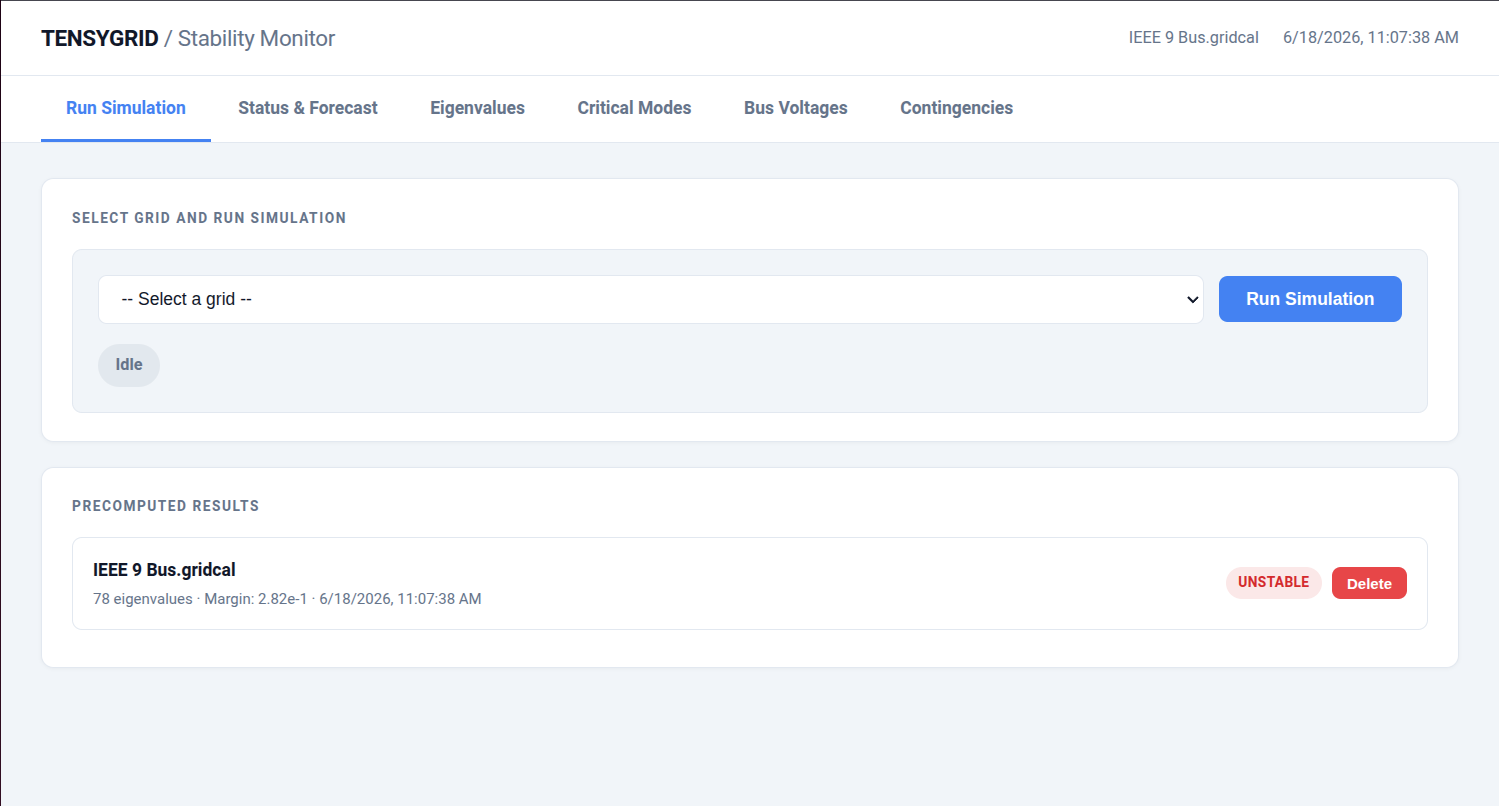
\includegraphics[width=0.7\textwidth]{pictures/UC-01.run_simulation.png}
          \caption[UC-01: Assessment of small-signal stability.]{UC-01: Assessment of small-signal stability under given operating conditions. The operator selects a grid model, runs the analysis, and monitors progress in the log panel. Upon completion, the result is stored and classified by stability status.}
        \end{figure}

  \item[GUI interaction.] The \textbf{Run Analysis} tab contains an input-source selector, action buttons (Run / Stop), a status badge, an execution log panel, and a list of previously computed results. File-based inputs display the detected format and any conversion warnings. IPSA and API-based sources additionally display connector status and validation results before the analysis starts. Each result item shows the analysis timestamp, the grid name, and the stability classification. A delete button allows removal of obsolete or failed results.
  \item[Expected result.] A \texttt{.tensygrid} file containing the full stability analysis output: eigenvalues, critical modes with participation factors, bus voltages from the power flow, grid topology information, the stability margin, and an operation hash for traceability. This file serves as input for all subsequent use cases (UC-02 to UC-05).
\end{description}




% ---------------------------------------------------------------------------
\subsection{UC-02: Monitoring and screening of power system small-signal stability margins}
% ---------------------------------------------------------------------------

\begin{description}
  \item[Actor.] Network operator; planning engineer or stability analyst for the detailed spectrum exploration.
  \item[Objective.] Obtain an immediate, general classification of grid stability together with key topological and operational metrics, and explore the full eigenvalue distribution in the complex plane to identify clusters, assess damping ratios, and detect modes of concern.
  \item[Preconditions.] At least one analysis (UC-01) has been completed and its result is loaded.
  \item[Theoretical basis.] Using UC-01 theoretical basis, we find different regimes in the system stability. We define the dominant eigenvalue $\lambda_1$ as the one with the biggest $\Re(\lambda)=\sigma$. For a sufficiently large time $t$, any other mode becomes negligible relative to the dominant one, since
        \[
          \frac{\mathrm{e}^{\lambda_n t}}{\mathrm{e}^{\lambda_1 t}}
          = \mathrm{e}^{(\lambda_n-\lambda_1)t} \xrightarrow[t\to\infty]{} 0 \quad \text{for } n\neq 1 \ \text{with } \sigma_1>\sigma_n .
        \]
        Therefore, if $\sigma_1>0$, the dominant term blows up to positive infinity, causing a clear instability, whereas $\sigma_1<0$ drives all modes to decay.

        These two verdicts are conclusive because, when no eigenvalue has $\Re(\lambda)=0$, the equilibrium is hyperbolic and the Hartman--Grobman theorem guarantees that, in a neighbourhood of the equilibrium, the nonlinear flow is topologically conjugate to its linearisation. The sign of $\sigma$ therefore reproduces the true local behaviour and not merely a first-order approximation. The theorem also marks the limit of the eigenvalue test: as soon as one mode reaches $\Re(\lambda)=0$, the equilibrium is non-hyperbolic, the linearisation is no longer topologically equivalent to the nonlinear flow, and the verdict has to come from higher-order terms (UC-13).

        The remaining singular case is a mode on the imaginary axis, $\Re(\lambda)=\sigma=0$, which may be a null eigenvalue ($\omega=0$) or a purely imaginary conjugate pair ($\lambda=\pm j\omega$, a Hopf-type mode): the argument above rests on the gap $\sigma_1-\sigma_n>0$, but here $\sigma_1=\sigma_n=0$ makes the exponent $\lambda_n-\lambda_1$ vanish, so the ratio does not tend to zero and the mode is not negligible relative to the dominant one. This equilibrium mode neither decays nor grows (it may oscillate with constant amplitude), i.e.\ a marginally stable regime that the dashboard classifies as \emph{yellow}.

        It is important, however, to distinguish this genuine marginal mode from spurious null eigenvalues that arise purely from the algebraic structure of the generalised eigenproblem $\lambda\mathbf{E}\mathbf{x}=\mathbf{A}\mathbf{x}$: whenever the leading matrix $\mathbf{E}$ (or the pencil $\lambda\mathbf{E}-\mathbf{A}$) is singular, the spectrum contains null eigenvalues that are not associated with any decaying, growing, or oscillating dynamic mode. These structural zeros must be identified and excluded before classifying the system, so that the \emph{yellow} verdict is reserved for actual marginal dynamics.

        In addition, each oscillation mode is represented by a conjugate pair of eigenvalues $\lambda=\sigma\pm j\omega$, where $\sigma$ governs decay-or-growth and $\omega$ the angular frequency, so that $f=\omega/(2\pi)$ is the frequency in Hz. In the complex plane, the ratio of $\sigma$ to $|\lambda|$ gives the damping ratio $\zeta=-\sigma/\lvert\lambda\rvert$, which equals the cosine of the mode's angle with the negative real axis: $\zeta=\cos\theta$. Constant-damping loci therefore appear as straight lines (cones) through the origin, which is precisely what the threshold lines used in the eigenvalue view (e.g.\ $\zeta=0$ and $\zeta=0.05$) represent. Modes close to the imaginary axis $\sigma\approx 0$ fall inside the low-damping cone and are flagged as the ones of concern; the spectrum is inspected to identify which modes concentrate the disturbance. This attribution, however, is the object of UC-03.
  \item[Possible bottlenecks.] To identify the origin of zero eigenvalues that lead to an inconclusive response.

  \item[Main flow.]
        \begin{enumerate}[before=\leavevmode, leftmargin=*]
          \item The operator navigates to the \textbf{Status} tab.
          \item A compact colour-coded badge displays the overall stability classification:
                \begin{itemize}[before=\leavevmode, leftmargin=*]
                  \item \textbf{Green} | Stable: all eigenvalues have negative real parts with sufficient damping.
                  \item \textbf{Yellow} | Marginal: the dominant real part lies within the configured numerical tolerance of the imaginary axis (currently $10^{-6}$), or some modes exhibit low damping ($\zeta < 0.05$).
                  \item \textbf{Red} | Unstable: at least one eigenvalue has a positive real part.
                \end{itemize}
          \item The \textbf{Grid Information} card shows the network topology: number of buses, generators, lines, loads, and transformers.
          \item The \textbf{Key Metrics} card reports the stability margin, the number of critical modes, the total eigenvalue count, and the number of state variables.
          \item A compact complex-plane eigenvalue plot provides a visual overview of the spectrum, with a red dashed line marking the stability boundary ($\Re(\lambda) = 0$).
          \item The \textbf{Stability Assessment} card presents a textual summary with colour-coded recommendations (e.g., ``All modes stable'', ``Caution: low damping detected'', or ``Warning: positive real parts; the system is unstable'').
          \item When a detailed exploration is required, the operator navigates to the \textbf{Eigenvalues} tab, where a full-page complex-plane scatter plot displays all eigenvalues: horizontal axis = real part $\sigma$, vertical axis = imaginary part $\omega$ (angular frequency). A red dashed vertical line marks the stability boundary ($\sigma = 0$).
          \item The operator can \textbf{scroll to zoom} and \textbf{drag to pan} across the plot, allowing inspection of dense clusters or outlying modes.
          \item Hovering over a point displays a tooltip with the eigenvalue's real part, imaginary part, frequency in Hz, and damping ratio $\zeta$.
          \item A \textbf{Damping vs.~Frequency} scatter plot shows $\zeta$ against frequency. Critical threshold lines at $\zeta = 0$ and $\zeta = 0.05$ are drawn for reference.
          \item A full \textbf{Eigenvalue Table} lists all eigenvalues in tabular form, sortable by real part, damping, or frequency.
          \item An \textbf{Info} button opens a modal overlay explaining how to interpret eigenvalue plots and damping ratios, targeted at operators who may not be familiar with small-signal analysis.
        \end{enumerate}

        \begin{figure}[H]
          \centering
          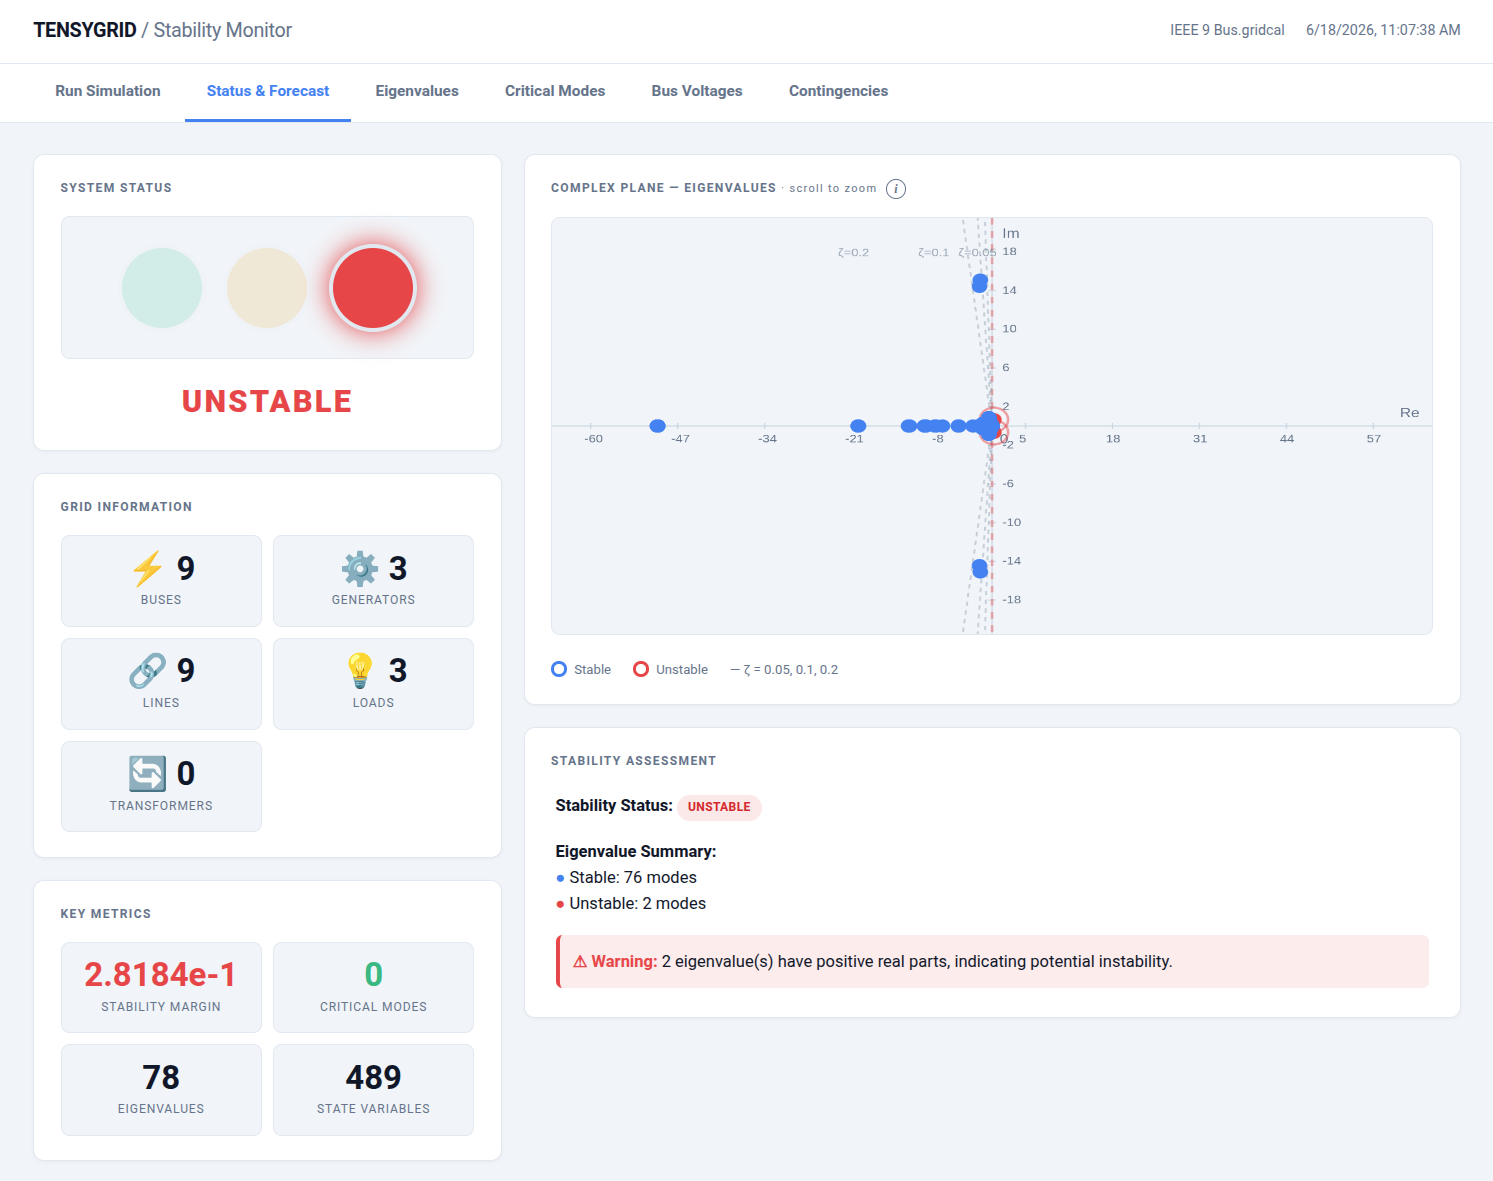
\includegraphics[width=0.7\textwidth]{pictures/UC-02.status_dashboard.png}
          \caption[UC-02: Status.]{UC-02: Status. The operator views the grid's stability status and related information in a consolidated dashboard.}
        \end{figure}

        \begin{figure}[H]
          \centering
          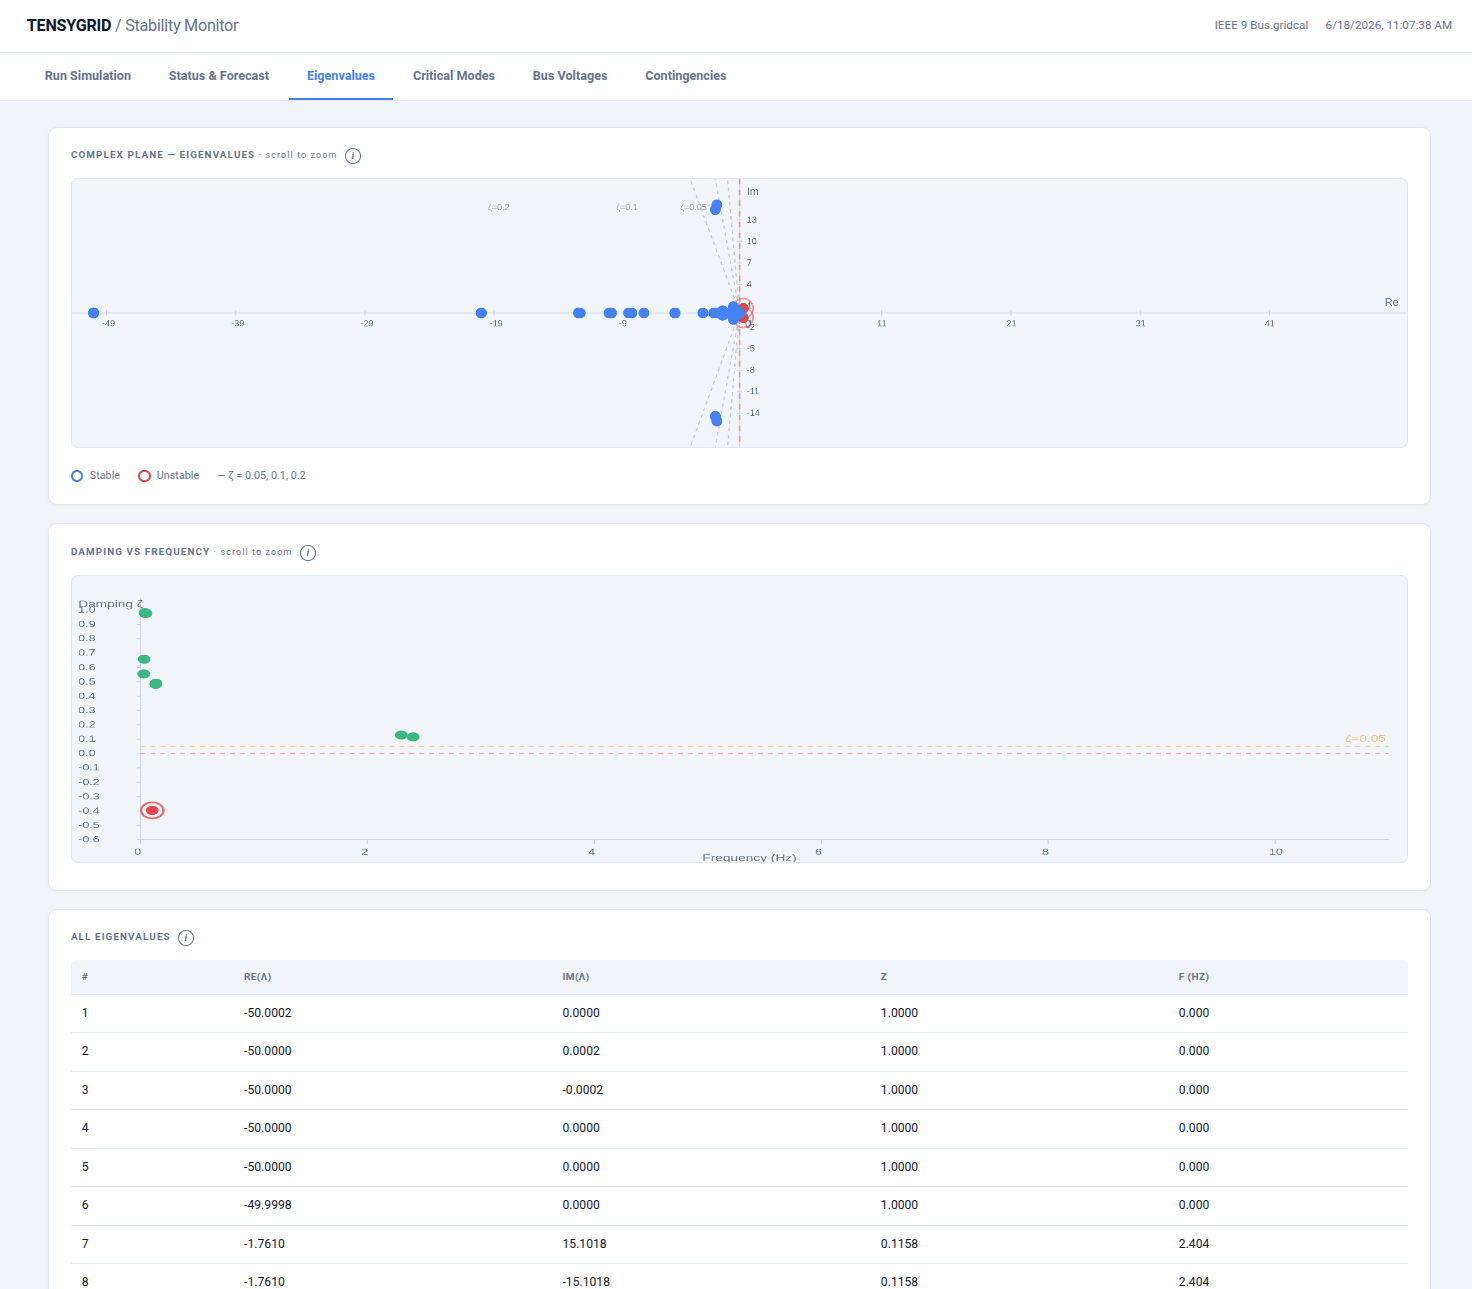
\includegraphics[width=0.7\textwidth]{pictures/UC-03.eigenvalues.png}
          \caption[UC-02: Eigenvalue analysis.]{UC-02: Eigenvalue analysis. The operator explores the eigenvalue distribution in the complex plane from the Eigenvalues tab.}
        \end{figure}

  \item[GUI interaction.] The \textbf{Status} tab is designed as a control-room dashboard. Colour-coded status badges draw the operator's attention to abnormal conditions without relying on animated traffic-light graphics. All metrics are displayed in large-format cards for quick scanning. The eigenvalue canvas of the \textbf{Eigenvalues} tab supports interactive zoom and pan via mouse or touch gestures. The damping plot and table are synchronised with the same data set and update when a different analysis result is loaded.
  \item[Expected result.] The operator obtains a clear answer to the question \textit{``Is the grid stable''?} together with enough context (topology, metrics) and a detailed understanding of the oscillatory modes (their frequencies, damping levels, and proximity to instability) to decide whether further investigation is needed. If the status is yellow or red, the operator is expected to proceed to UC-03 for detailed diagnosis of the critical modes, and uses this view to evaluate the effectiveness of remedial measures in contingency scenarios (UC-05).
\end{description}

% ---------------------------------------------------------------------------
\subsection{UC-03: Identification and diagnosis of critical oscillatory modes}
% ---------------------------------------------------------------------------

\begin{description}
  \item[Actor.] Stability engineer or control designer.
  \item[Objective.] Identify the least-damped oscillation modes and determine which state variables (generators, controls, components) contribute most to each mode.
  \item[Preconditions.] An analysis (UC-01) has been completed. Eigenvalues have been computed.
  \item[Theoretical basis.] Each eigenvalue corresponds to an oscillation mode that is a specific combination of perturbations in the state vector. The modal participation factor is defined as
        \[
          p_{ki}=\frac{v_{ki}\,(\mathbf{w}_k^{\top}\mathbf{E})_i}{\mathbf{w}_k^{\top}\mathbf{E}\,\mathbf{v}_k},
        \]
        where $\mathbf{v}_k$ and $\mathbf{w}_k$ are the right and left eigenvectors of the pencil $\lambda\mathbf{E}\mathbf{x}=\mathbf{A}\mathbf{x}$ (with $\mathbf{A}\mathbf{v}_k=\lambda_k\mathbf{E}\mathbf{v}_k$, $\mathbf{w}_k^{\top}\mathbf{A}=\lambda_k\mathbf{w}_k^{\top}\mathbf{E}$), $v_{ki}=\mathbf{e}_i^{\top}\mathbf{v}_k$ and $(\mathbf{w}_k^{\top}\mathbf{E})_i=\mathbf{w}_k^{\top}\mathbf{E}\,\mathbf{e}_i$~\cite{tzounas2019modal}. The GUI displays normalised magnitudes
        \[
          \bar{p}_{ki}=\frac{\lvert p_{ki}\rvert}{\sum_{j}\lvert p_{kj}\rvert},
        \]
        which sum to 100\% per mode. A large $\bar{p}_{ki}$ indicates that the $k$-th mode is strongly associated with the $i$-th state, making it a primary candidate for intervention (PSS retuning, FACTS placement).
  \item[Possible bottlenecks.] In sparse computations of the eigenvalues is difficult to compute their corresponding left and right eigenvectors that are both needed for this UC.
  \item[Main flow.]
        \begin{enumerate}[before=\leavevmode, leftmargin=*]
          \item The operator navigates to the \textbf{Critical Modes} tab.
          \item A table lists the modes with the lowest damping ratios, sorted from most to least critical. Each row shows the mode index, real part, imaginary part, frequency, damping ratio, and a stability badge.
          \item The operator clicks on a mode row to expand its \textbf{participation factors}.
          \item An inline bar chart displays the relative participation of each state variable: bars are proportional to the magnitude of the participation factor, and the state variable name is shown alongside.
          \item State variables associated with the same physical device (e.g., generator speed $\Delta\omega$, rotor angle $\Delta\delta$, AVR states) are visually grouped.
          \item The operator can identify which generators or components dominate the mode, helping to target power system stabiliser (PSS) tuning or FACTS placement at the most effective locations.
        \end{enumerate}

        \begin{figure}[H]
          \centering
          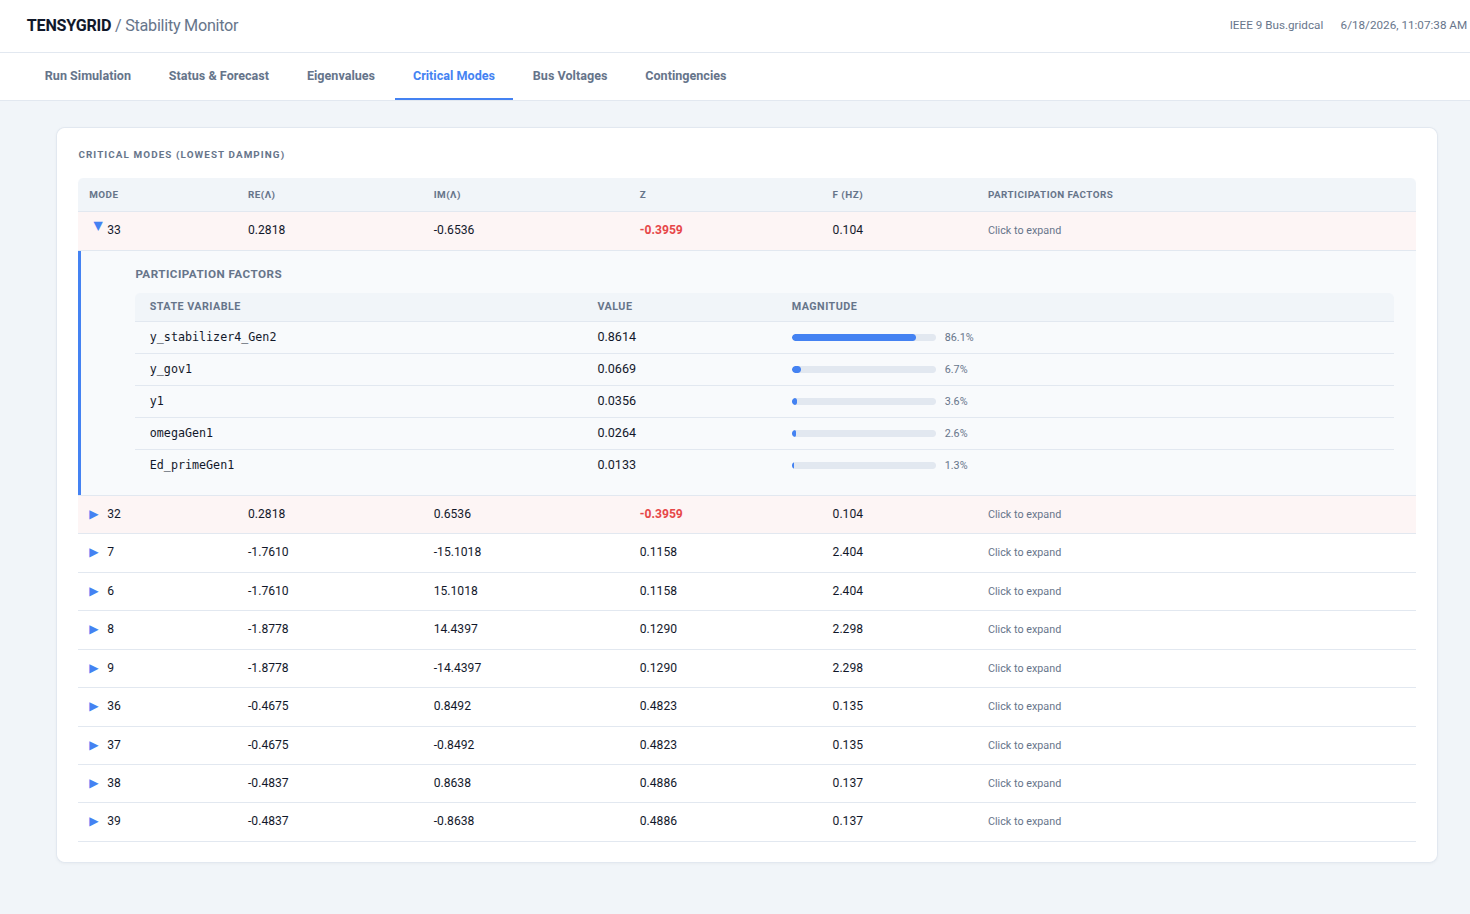
\includegraphics[width=0.7\textwidth]{pictures/UC-04.critical_modes.png}
          \caption[UC-03: Critical modes.]{UC-03: Critical modes. The operator identifies the least-damped oscillation modes.}
        \end{figure}
  \item[GUI interaction.] Participation factors are rendered as horizontal bar charts inside expandable table rows. The expansion is animated. The operator can collapse a row and expand another to compare participation profiles across different modes.
  \item[Expected result.] The operator learns \textit{which physical components are responsible for each critical oscillation}. For example, Mode 3 with $\zeta = 0.02$ at 1.2 Hz may show strong participation from Generator 7's speed and AVR states, indicating that retuning the PSS at that generator would be the most effective mitigation. This directly informs the decisions proposed in next use cases.
\end{description}

% ---------------------------------------------------------------------------
\subsection{UC-04: Assessment of bus voltage profiles and operating limit violations}
% ---------------------------------------------------------------------------

\begin{description}
  \item[Actor.] Network operator.
  \item[Objective.] Verify that the voltage magnitudes obtained from the power-flow solution are within acceptable operating limits.
  \item[Preconditions.] An analysis (UC-01) has been completed and the power-flow solution is available.
  \item[Theoretical basis.] The power-flow solution provides the steady-state voltage magnitude and angle at each bus of the network. The per-unit voltage magnitude $V_\mathrm{p.u.}$ is compared against operational limits: normal operating range (e.g.\ $0.95$--$1.05$ p.u.) and emergency limits (e.g.\ $0.90$--$1.10$ p.u.). Buses outside the normal range but within emergency limits are flagged as WARNING; buses beyond emergency limits indicate a severe violation. UC-04 does not perform an iMTI calculation independently. It reuses the operating-point power flow already required by UC-01 and complements the eigenvalue-based assessment, because a system can be small-signal stable while exhibiting unacceptable voltage profiles.
  \item[Main flow.]
        \begin{enumerate}[before=\leavevmode, leftmargin=*]
          \item The operator navigates to the \textbf{Bus Voltages} tab.
          \item A table lists every bus in the network with its name (or index) and its voltage magnitude in per-unit (p.u.).
          \item Each bus row carries a colour-coded status badge:
                \begin{itemize}[before=\leavevmode, leftmargin=*]
                  \item \textbf{OK} (green) | voltage is within the normal operating range (e.g., $0.95$--$1.05$ p.u.).
                  \item \textbf{WARNING} (orange) | voltage is outside the normal range but within emergency limits (e.g., $0.90$--$1.10$ p.u.).
                \end{itemize}
          \item Buses with WARNING status are flagged for operator attention. The operator can sort the table by voltage magnitude to quickly locate under-voltage or over-voltage buses.
        \end{enumerate}

        \begin{figure}[H]
          \centering
          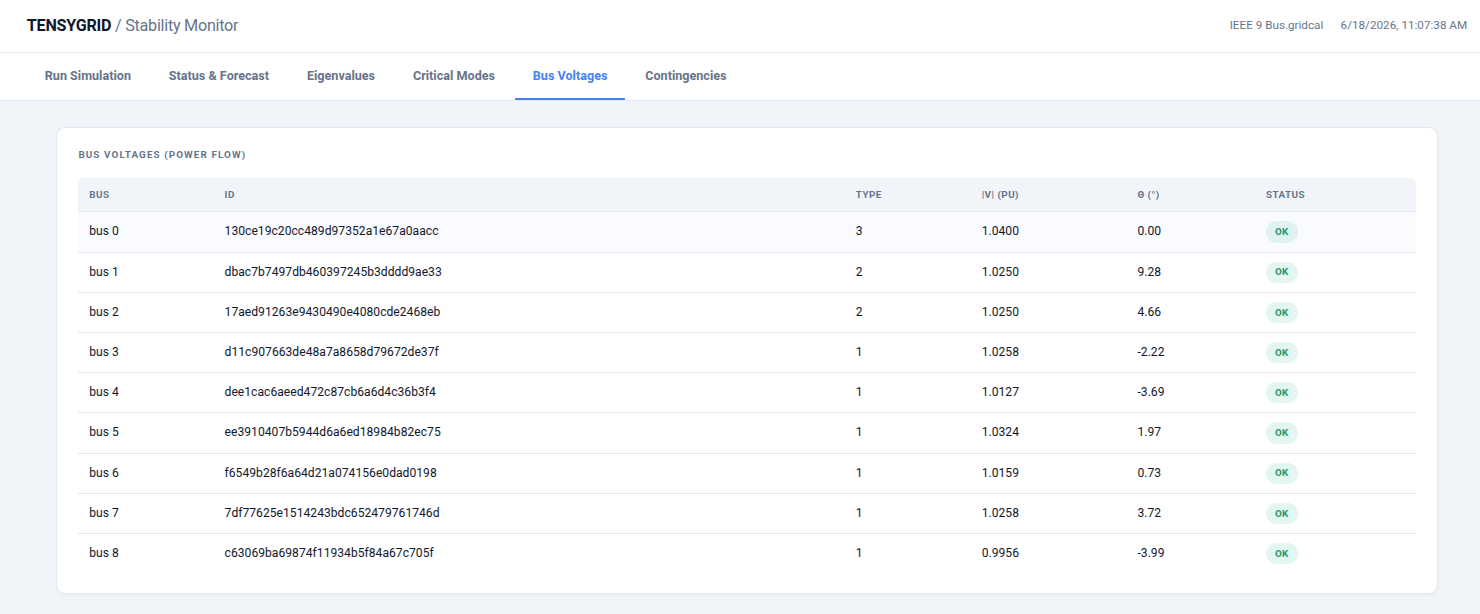
\includegraphics[width=0.7\textwidth]{pictures/UC-05.bus_voltages.png}
          \caption[UC-04: Bus voltage assessment.]{UC-04: Bus voltage assessment. The operator validates the voltage profile under the current operating point.}
        \end{figure}
  \item[GUI interaction.] The bus voltage table is a scrollable table with sortable columns. The OK/WARNING badges use the same colour semantics as the stability traffic lights, maintaining visual consistency across the interface.
  \item[Expected result.] The operator obtains a quick validation of the voltage profile under the current operating point. Buses with voltage excursions are highlighted, prompting further investigation into reactive power support, tap-changer settings, or load behaviour.
\end{description}



% ---------------------------------------------------------------------------
\subsection{UC-05: Identification of stability risks under $N-1$ contingencies}
% ---------------------------------------------------------------------------

\begin{description}
  \item[Actor.] Network operator or planning engineer.
  \item[Objective.] Evaluate the impact of a single-element outage (generator, line, or load) on the small-signal stability of the grid.
  \item[Preconditions.]
        \begin{itemize}[before=\leavevmode, leftmargin=*]
          \item A base-case analysis (UC-01) has been completed and serves as the pre-contingency reference.
          \item The grid model contains the values of the element to be removed.
        \end{itemize}
  \item[Theoretical basis.] For each selected outage, the affected device is changed from \texttt{active} to \texttt{inactive}. A new power flow determines the post-contingency equilibrium, after which the iMTI descriptor matrices and eigenvalues are recomputed. The use case is therefore not a conventional $N-1$ power-flow check alone: its TenSyGrid contribution is the comparison of pre- and post-contingency small-signal stability margins and critical modes.
  \item[Main flow.]
        \begin{enumerate}[before=\leavevmode, leftmargin=*]
          \item The operator navigates to the \textbf{Contingencies} tab.
          \item The operator selects the contingency type from a dropdown: \textbf{Generator}, \textbf{Line}, or \textbf{Load}.
          \item A second dropdown is populated with the available elements of the selected type (e.g., "Generator 0", "Line 3"). The operator selects the specific element to be removed.
          \item The operator clicks the \textbf{Analyse Contingency} button.
          \item The backend launches the contingency analysis script, which removes the selected element from the grid model, re-computes the power flow and the small-signal stability, and returns the post-contingency eigenvalues.
          \item The results are displayed as a side-by-side comparison: two complex-plane eigenvalue plots (pre-contingency vs.~post-contingency) sharing the same axis scales, plus a summary table listing the contingency type, the element removed, and the change in stability margin.
          \item The tool generates \textbf{automatic recommendations} based on the observed change:
                \begin{itemize}[before=\leavevmode, leftmargin=*]
                  \item If the system becomes unstable: ``Consider installing PSS at the most participating generators or adding a STATCOM/SVC near the affected bus''
                  \item If damping degrades below the 5\% threshold: ``Low-damped modes detected; evaluate PSS retuning or FACTS placement''
                  \item If the stability margin decreases significantly: ``Re-dispatch generation or reinforce the affected corridor to recover margin''
                \end{itemize}
          \item The operator can repeat the analysis for different elements to explore multiple $N-1$ scenarios. A \textbf{Stop} button is available to cancel a running contingency analysis if it takes too long.
        \end{enumerate}
        \begin{figure}[H]
          \centering
          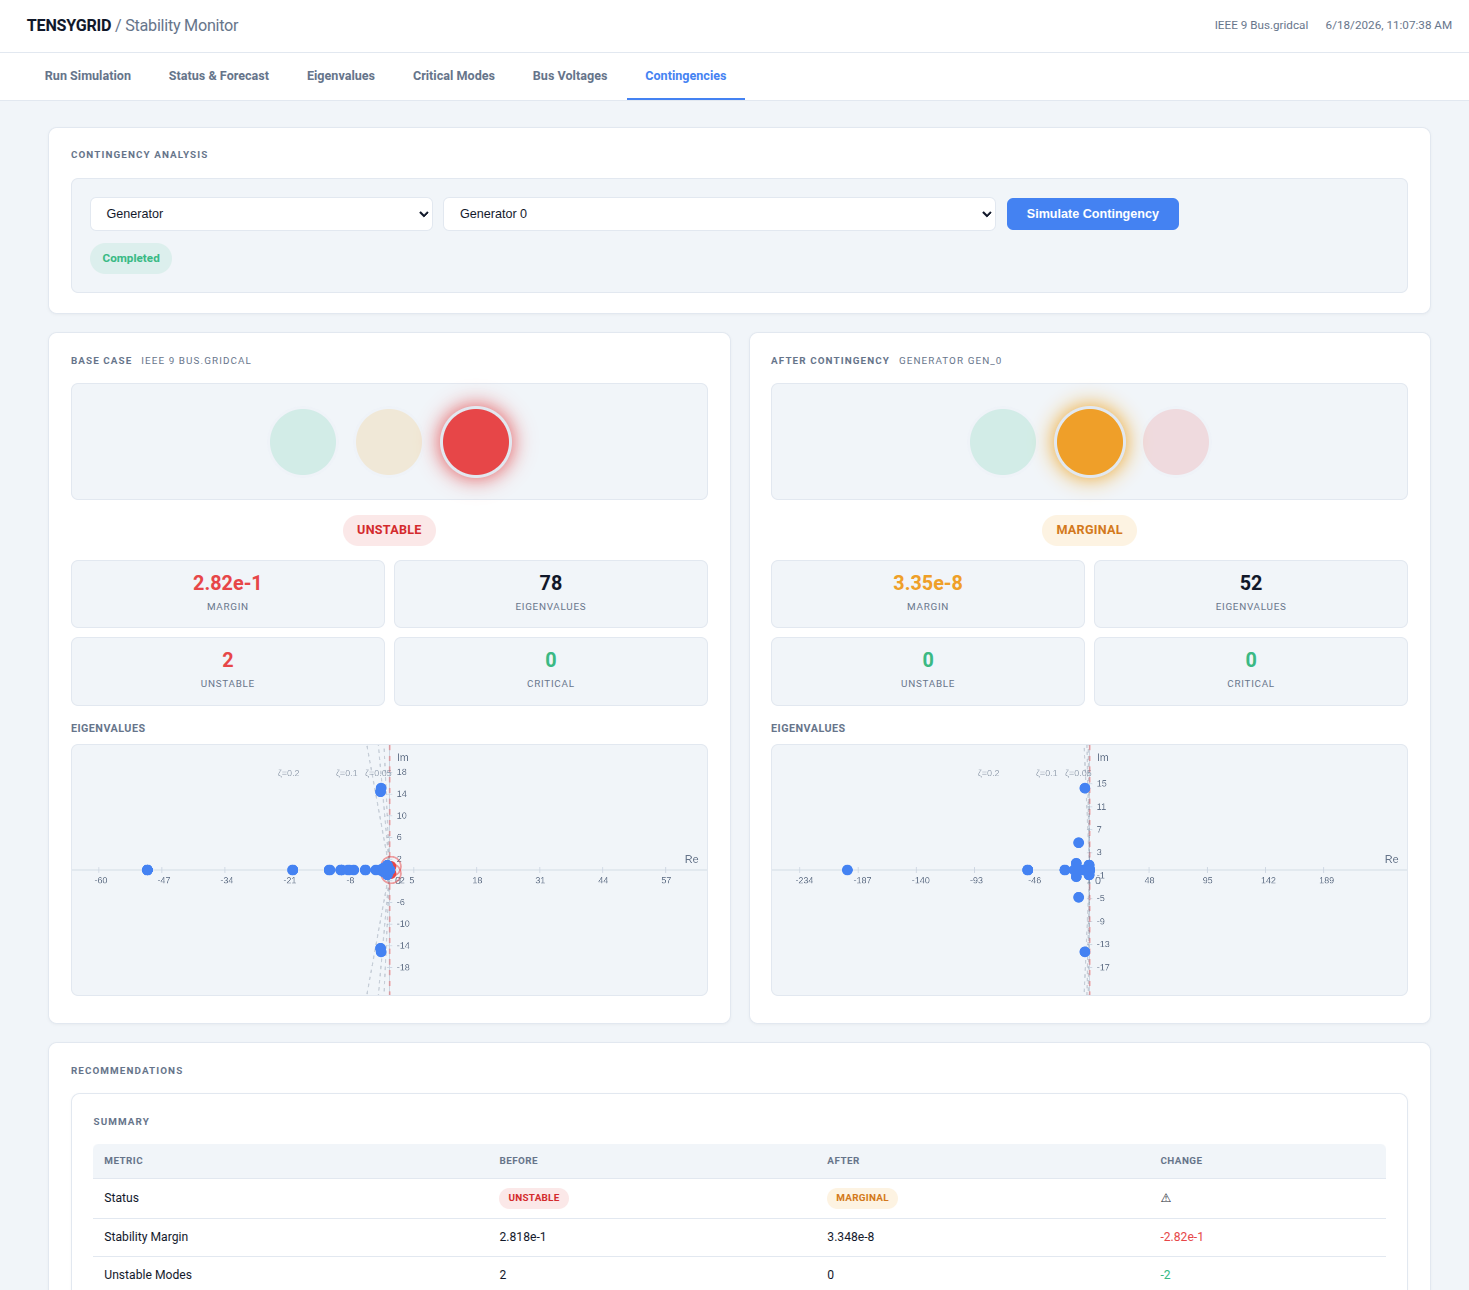
\includegraphics[width=0.7\textwidth]{pictures/UC-06.contingencies.png}
          \caption[UC-05: Contingency analysis.]{UC-05: Contingency analysis. The operator evaluates the impact of different contingencies on system stability.}
        \end{figure}
  \item[GUI interaction.] The Contingencies tab uses a three-column layout: controls on the left, eigenvalue comparison in the centre, and recommendations on the right. The before/after plots share the same axis scales for direct visual comparison.
  \item[Expected result.] The operator determines whether the grid remains stable under the selected $N-1$ contingency. If instability or marginal stability is detected, the operator receives targeted, actionable recommendations. This use case supports transmission planning studies and operational security assessment, enabling the operator to identify critical contingencies and plan mitigation measures.
\end{description}


\section{Proposed use cases}

The five use cases described in the previous section correspond to functionalities already prototyped in the Stability Monitor. The following nine use cases are proposed extensions derived from industry interviews, internal technical discussions, or the extension of implemented features. They address workflows that may be relevant to planning and operational studies but remain subject to consortium prioritisation. UC-13 and UC-14 are the most research-oriented proposals and are included so that their assumptions and feasibility can be assessed early.

% ---------------------------------------------------------------------------
\subsection{UC-06: Comparative stability assessment across operating scenarios}
% ---------------------------------------------------------------------------

% \begin{description}
%   \item[Actor.] Network operator or planning engineer.
%   \item[Objective.] Compare the stability characteristics of two distinct grid operating points, such as summer peak vs.\ winter off-peak, high vs.\ low renewable generation, or pre- and post-reinforcement scenarios.
%   \item[Proposed flow.] The operator loads two previously computed \texttt{.tensygrid} results. The tool renders side-by-side eigenvalue plots, a table comparing key metrics (margin, critical mode count, lowest damping), and highlights modes that appear or disappear between the two scenarios. Differences in participation factors are flagged to identify shifts in the dominant oscillatory behaviour.
%   \item[Expected value.] Operators can assess how seasonal, daily, or structural changes in the network affect stability without manually switching between result sets. This supports both operational planning and infrastructure investment decisions.
% \end{description}

\begin{description}
  \item[Actor.] Network operator or planning engineer.
  \item[Objective.] Compare the stability characteristics of two distinct grid operating points, such as day peak vs.\ night off-peak, high vs.\ low renewable generation, or pre- and post-reinforcement scenarios.
  \item[Proposed flow.] The operator loads two previously computed \texttt{.tensygrid} results. The tool performs a differential modal analysis, directly mapping eigenvalues between the two states to track modal shifts. It renders comparative plots and highlights critical structural changes: modes that emerge or disappear, significant drops in damping, and shifts in participation factors that indicate the oscillatory problem has relocated geographically.
  \item[Expected value.] Operators can assess how seasonal, daily, or structural changes in the network affect stability without manually switching between result sets. This supports both operational planning and infrastructure investment decisions.
\end{description}

% ---------------------------------------------------------------------------
\subsection{UC-07: Identification of devices contributing to stability issues}
% ---------------------------------------------------------------------------

\begin{description}
  \item[Actor.] Planning engineer.
  \item[Objective.] Rank the devices of the network by their participation in the critical modes, so that the equipment that most affects the stability of the system can be identified and prioritised.
  \item[Preconditions.]
        \begin{itemize}[before=\leavevmode, leftmargin=*]
          \item An analysis (UC-01) has been completed and the critical modes have been diagnosed (UC-03).
          \item The participation factors of the state variables are available in the result file.
        \end{itemize}
  \item[Theoretical basis.] Each participation factor relates a state variable to a critical mode, so the variables with the largest participation identify the dynamics that dominate that mode. Mapping each state variable onto the device that owns it (generator, AVR, PSS, converter, load) and aggregating the participation factors per device yields a ranking that links every critical eigenvalue to the physical equipment responsible for it. This is the step from the state-level diagnosis of UC-03 to a device-level decision.
  \item[Possible bottlenecks.] The aggregation is only as good as the metadata that maps states to devices, and several choices must be made explicit:
        \begin{itemize}[before=\leavevmode, leftmargin=*]
          \item \textbf{State-to-device mapping.} The result file must retain which device owns each state; otherwise the mapping has to be reconstructed from the model.
          \item \textbf{Aggregation criterion.} Summing the participation factors of all the states of a device favours devices with many states, whereas taking the maximum ignores their combined effect, so the criterion must be configurable.
          \item \textbf{Normalisation and operating point.} Participation factors depend on the mode normalisation and on the operating point, so the ranking may change between scenarios and should be reported with that caveat.
          \item \textbf{Number of critical modes.} A ranking per mode is easy to read, but a global ranking across the critical modes requires weighting them by criticality.
        \end{itemize}
  \item[Proposed flow.]
        \begin{enumerate}[before=\leavevmode, leftmargin=*]
          \item The operator selects a result and the critical mode to inspect.
          \item The tool groups the state variables by owning device and aggregates their participation factors with the selected criterion.
          \item A table ranks the devices by aggregated participation, and a bar chart shows their relative weight in the mode.
          \item The operator can expand a device to see the state-level participation factors behind its position in the ranking, and switch between the per-mode and the global views.
          \item The ranking can be exported as the starting point for the controller-placement analysis of UC-10.
        \end{enumerate}
  \item[Expected value.] The planning engineer obtains a device-level list that translates the modal diagnosis into concrete equipment priorities: which generators, controls, or loads dominate each critical mode and therefore concentrate the mitigation effort. This supports maintenance and retuning plans, the siting of PSS or FACTS devices, and the discussion with asset managers about where stability investment is most effective.
\end{description}

% ---------------------------------------------------------------------------
\subsection{UC-08: Assessment of stability margins under increasing system loading}
% ---------------------------------------------------------------------------

% \begin{description}
%   \item[Actor.] Network operator or planning engineer.
%   \item[Objective.] Track the evolution of the stability margin across a sequence of operating points, such as a daily load curve, a weekly dispatch schedule, or a time series of snapshots from a historical database.
%   \item[Proposed flow.] The operator selects a set of precomputed results (ordered by time or by a parameter such as total demand). The tool plots the stability margin and the damping of the most critical mode as a function of the ordering parameter. A threshold line indicates when the margin enters the marginal or unstable region, enabling early warning of degradation trends.
%   \item[Expected value.] Operators can identify \textit{when} during the day or the year the grid is most vulnerable, and at which operating condition proactive measures (e.g., generation re-dispatch) should be considered.
% \end{description}

\begin{description}
  \item[Actor.] Network operator or planning engineer.
  \item[Objective.] Track the evolution of the stability margin near an operating point, bridging both static and dynamic stability dimensions, to evaluate maximum loadability and proactively anticipate the need for a full Continuation Power-Flow (CPF) study.
  \item[Proposed flow.] The operator selects a precomputed operating state. By utilizing sensitivity analysis or linearizations of the Jacobian matrix, the tool extrapolates nearby critical points before they are reached in real-world operation. Bridging both static and dynamic stability perspectives, the system simultaneously plots the voltage stability margin (static) and the damping ratio of the most critical electromechanical mode (dynamic) obtained via eigenvalue analysis as a function of the loading parameter. A configurable threshold line indicates when either margin enters a marginal or unstable region, triggering an early warning that a full CPF study or preventive actions are required.
  \item[Expected value.] Operators gain a unified, comprehensive view of grid vulnerability. They can identify specific windows (e.g., peak hours or seasonal conditions) and determine exactly at which operating thresholds proactive measures, such as generation re-dispatch or topology changes, must be deployed before dynamic oscillations or voltage collapse compromise the system.
\end{description}

% ---------------------------------------------------------------------------
\subsubsection{Online monitoring variant of UC-08}
% ---------------------------------------------------------------------------


\begin{description}
  \item[Actor.] Network operator or planning engineer.
  \item[Objective.] Extend UC-08 to track, in near real time, whether the grid is approaching a critical operating point along a previously analysed trajectory.
  \item[Proposed flow.] The operator selects a precomputed result of critical paths from UC-08. The tool then checks if the current operating point is approaching any of the critical points identified in the previous use case. The system continuously monitors the stability margin and the damping ratio of the most critical mode, providing real-time feedback on the grid's stability status. If the system detects that the grid is approaching a critical point, it triggers an alert to notify the operator.
  \item[Expected value.] This optional UC-08 workflow improves situational awareness by comparing the current operating point with precomputed critical paths. It does not imply that the present prototype already provides production-grade real-time integration.
\end{description}

% ---------------------------------------------------------------------------
\subsection{UC-09: Ranking of critical system elements affecting stability}
% ---------------------------------------------------------------------------

\begin{description}
  \item[Actor.] Network operator, planning engineer, or asset manager.
  \item[Objective.] Rank generators, lines, and loads by their individual contribution to stability degradation, going beyond single $N-1$ analysis.
  \item[Proposed flow.] The operator triggers a batch contingency analysis ($N-1$ or $N-2$) across all elements of a selected type. For each contingency, the change in stability margin is recorded. The tool then produces a ranked bar chart or heat map showing which elements cause the largest margin reduction when removed. The operator can click on any element to drill down into the detailed contingency result (as in UC-05).
  \item[Expected value.] This use case transforms contingency analysis from a \textit{what-if} exploration into a systematic vulnerability assessment. It directly supports critical-asset identification, maintenance prioritisation, and transmission expansion planning.
\end{description}

% ---------------------------------------------------------------------------
\subsection{UC-10: Identification of suitable locations for damping controller installation}
% ---------------------------------------------------------------------------

\begin{description}
  \item[Actor.] Stability engineer or control designer.
  \item[Objective.] Provide two clearly separated mitigation pathways for low-damped modes: retuning existing controllers and assessing candidate locations for new damping equipment.
  \item[Proposed flow.]
        \begin{enumerate}[before=\leavevmode, leftmargin=*]
          \item Building on UC-03 and UC-07, the tool analyses participation factors, residues, modal observability, and controllability across the base operating point and selected contingencies.
          \item \textbf{Existing-controller retuning path.} The tool identifies generators or converters whose installed PSS or damping controls have high influence on the critical mode. It ranks them as candidates for a subsequent parameter-tuning study, without claiming to calculate the optimal gains or time constants.
          \item \textbf{New-device placement path.} If existing controls do not provide an adequate mitigation path, the tool ranks candidate buses for new PSS-equipped generation or FACTS devices (STATCOM, SVC, or TCSC). This output is explicitly presented as a capital-investment option requiring a separate techno-economic study.
          \item The GUI reports the two rankings in separate panels and labels the evidence, assumptions, and expected qualitative effectiveness of each recommendation.
        \end{enumerate}
  \item[Expected value.] Operators and engineers can distinguish a comparatively low-cost controller-retuning study from the installation of new equipment. The use case translates modal diagnostics into actionable alternatives without implying that the two decisions have the same cost, approval process, or implementation horizon.
\end{description}

% ---------------------------------------------------------------------------
\subsection{UC-11: Assessment of renewable energy integration impact on system stability}
% ---------------------------------------------------------------------------

\begin{description}
  \item[Actor.] Planning engineer or policy analyst.
  \item[Objective.] Evaluate the small-signal stability of the grid under different renewable energy penetration scenarios, assessing how the progressive substitution of synchronous generation by converter-interfaced resources affects system stability.
  \item[Preconditions.]
        \begin{itemize}[before=\leavevmode, leftmargin=*]
          \item A base-case analysis (UC-01) has been completed and serves as the reference operating point.
          \item The grid model identifies which machines are synchronous generators and which are converter-interfaced resources, so that the generation mix can be modified without altering the network topology.
          \item At least one converter-interfaced generator model (e.g.\ GFL or GFM) is available to replace the synchronous machines that are scaled down.
        \end{itemize}
  \item[Theoretical basis.] A synchronous generator is described by the swing equation together with the flux and control dynamics of the machine, whereas a complete model of an inverter-based generator adds the converter's inner current and voltage control, the phase-locked loop (or grid-forming virtual impedance), and any outer power or DC-link dynamics. The interface variables exchanged with the network remain the same: the current or power injected at the connection bus. Substituting synchronous machines by converters changes the number and nature of the internal states, so the descriptor matrices $\mathbf{E}$ and $\mathbf{A}$ of the pencil $\lambda\mathbf{E}\mathbf{x}=\mathbf{A}\mathbf{x}$ grow and change shape. Consequently, electromechanical modes of the displaced synchronous machines fade while new converter-driven modes appear. Evaluating the margin and critical modes as a function of penetration exposes this transition.
  \item[Possible bottlenecks.] Substituting the device equations changes the shape of the $\mathbf{E}$ and $\mathbf{A}$ matrices, so the assembly and pre-processing chain must adapt to a spectrum that mixes synchronous and converter states. Code optimisation may require a complete iteration of the software, and the outcome depends on the accuracy of the converter models, which must be agreed upon before scenarios can be compared.
  \item[Proposed flow.]
        \begin{enumerate}[before=\leavevmode, leftmargin=*]
          \item The operator selects a base-case result (UC-01) and defines a set of penetration scenarios (e.g.\ 30\%, 50\%, 70\%, 100\% of inverter-based generation), optionally together with a set of critical contingencies.
          \item For each scenario, the tool adjusts the generation mix by scaling down synchronous machines and scaling up converter-interfaced sources while respecting the grid model's structure. It then runs the stability analysis and records the stability margin and critical modes.
          \item Results are presented as a curve of stability margin versus renewable penetration, with flags for the penetration level at which the margin crosses the marginal or unstable threshold.
          \item Eigenvalue trajectories are plotted to show how specific modes migrate as the penetration level increases, with the newly introduced converter modes highlighted.
          \item Critical scenarios can be drilled down via UC-03 (participation factors) and tracked along the progression via UC-08.
        \end{enumerate}
  \item[Expected value.] This use case directly addresses the core TenSyGrid objective of assessing converter-dominated grids. It allows grid planners to determine the maximum renewable hosting capacity under stability constraints and to identify the modes most sensitive to the synchronous-to-converter transition.
\end{description}

% ---------------------------------------------------------------------------
\subsection{UC-12: Automated documentation and reporting of stability assessment results}
% ---------------------------------------------------------------------------

\begin{description}
  \item[Actor.] Network operator, planning engineer, or regulatory compliance officer.
  \item[Objective.] Produce a self-contained stability assessment report in a standardised, exportable format (PDF or HTML) suitable for internal documentation, regulatory submission, or stakeholder communication.
  \item[Proposed flow.] The operator selects one or more analysis results and a report template (e.g., \textit{Standard Stability Assessment}, \textit{Contingency Analysis Summary}, or \textit{Renewable Integration Study}). The tool compiles the following sections in the background: (i) executive summary with stability classification; (ii) grid topology and operating-point description; (iii) eigenvalue plot and critical-mode table; (iv) contingency-analysis results, if available; and (v) recommendations. The report includes the operator's logo, author name, date, and a disclaimer. The operator can preview the report before exporting.
  \item[Expected value.] Automating report generation reduces the manual effort required to document stability studies, ensures consistency across assessments, and facilitates communication with non-technical stakeholders (regulators, management, public authorities).
\end{description}

% ---------------------------------------------------------------------------
\subsection{UC-13: Assessment of nonlinear system behaviour near critical operating points}
% ---------------------------------------------------------------------------

\begin{description}
  \item[Actor.] Stability engineer or control designer.
  \item[Objective.] Determine the local behaviour of the equilibrium when the linearised model exhibits zero (or near-zero) eigenvalues, by reducing the dynamics onto the centre manifold, so that the tool can distinguish genuine marginal modes from structural zeros and report whether the equilibrium is attracting, repelling, or incipiently bifurcating.
  \item[Preconditions.]
        \begin{itemize}[before=\leavevmode, leftmargin=*]
          \item An analysis (UC-01) has been completed and its result is loaded.
          \item The spectrum contains eigenvalues with $\sigma = 0$ (or $\lvert\sigma\rvert$ below a configurable tolerance).
          \item Structural null eigenvalues arising from a singular pencil $\lambda\mathbf{E}-\mathbf{A}$ have been identified and excluded, as required by UC-02.
        \end{itemize}
  \item[Theoretical basis.] The Hartman--Grobman theorem guarantees that the linearisation reproduces the local behaviour of the nonlinear system only when the equilibrium is hyperbolic, i.e.\ when every eigenvalue satisfies $\Re(\lambda)\neq 0$. When an eigenvalue lies on the imaginary axis, either as a real zero (saddle-node) or a purely imaginary conjugate pair (Hopf), the theorem does not apply, the linear model is inconclusive, and the Centre Manifold Theorem (CMT) must be used instead. Before computing the invariant sub-manifolds, an ODE must be obtained from the differential-algebraic (DAE) formulation so that structural zeros caused by a singular $\mathbf{E}$ are discarded. Given the centre subspace $\mathcal{E}^{c}=\operatorname{span}\{\mathbf{v}_i:\lambda_i=0\}$ and a complementary stable subspace $\mathcal{E}^{s}$, the state can be split as $\mathbf{x}=\mathbf{x}_0+q+p$ (with $q\in\mathcal{E}^{c}$, $p\in\mathcal{E}^{s}$). An invariant graph $p=h(q)$, tangent to $\mathcal{E}^{c}$ at the equilibrium, yields reduced dynamics $\dot{q}=g(q)$ that govern the local behaviour. The first non-vanishing term of $g$ classifies the equilibrium and helps identify the associated bifurcation.
  \item[Possible bottlenecks.] Deriving an equivalent ODE from the DAE is not as trivial as it may seem. Although one could consider rewriting the algebraic constraints as generalised coordinates, in the spirit of Hamiltonian systems, this is not feasible in the present setting. An alternative is index reduction by repeated differentiation, which fits the proposed multilinear methodology but whose scaling behaviour on large systems is still unknown. Direct approaches based on Gaussian elimination (e.g.\ for the structural analysis of the descriptor) could also be explored, but it is not suitable for sparse matrices since it could break that behaviour.
  \item[Proposed flow.]
        \begin{enumerate}[before=\leavevmode, leftmargin=*]
          \item The operator selects a result containing zero or near-zero eigenvalues and opens the \textbf{Centre Manifold} view.
          \item The tool separates structural zeros (singular pencil) from genuine equilibrium modes and reports which ones are retained, so that the \emph{yellow} verdict of UC-02 can be justified rather than assumed.
          \item For the retained modes, the tool computes the centre manifold reduction and returns the leading normal-form coefficient together with its sign.
          \item The equilibrium is classified as asymptotically stable, unstable, or semistable on the centre manifold, and the associated bifurcation type and critical parameter direction are reported.
          \item A one-dimensional phase portrait of the reduced flow $\dot{x}_c=g(x_c)$ is plotted, showing the equilibrium and the direction of the trajectories.
          \item If the coefficient is close to zero (degenerate case), the tool flags the result as inconclusive and recommends computing higher-order terms or moving the operating point.
        \end{enumerate}
  \item[Expected value.] The operator or engineer resolves the ambiguity left by a null eigenvalue: instead of a generic \emph{yellow} status, the tool states whether the operating point is a benign equilibrium, an incipient bifurcation, or an artefact of the descriptor formulation. This feeds the recommendation logic of UC-05 and clarifies which parameter (load, dispatch, penetration) must be watched before the equilibrium disappears.
\end{description}

% ---------------------------------------------------------------------------
\subsection{UC-14: Assessment of the region of attraction following system disturbances}
% ---------------------------------------------------------------------------

\begin{description}
  \item[Actor.] Planning engineer or security analyst.
  \item[Objective.] Estimate the region of the state space from which the system returns to the current operating point after a disturbance, and express it as an interpretable security margin (e.g.\ maximum tolerable disturbance magnitude or critical clearing time) for a user-selected family of disturbances.
  \item[Preconditions.]
        \begin{itemize}[before=\leavevmode, leftmargin=*]
          \item An analysis (UC-01) has been completed and the equilibrium, state matrix, and tensor expansion are available.
          \item The equilibrium is hyperbolic and small-signal stable (all $\sigma<0$); if some mode has $\sigma>0$ the basin is empty and the tool reports the instability directly, whereas a mode with $\sigma=0$ is non-hyperbolic and is redirected to UC-13.
          \item A family of disturbances has been defined (fault location and clearing time, or a load/generation step at a given bus).
        \end{itemize}
  \item[Theoretical basis.] Eigenvalue analysis certifies only \emph{local} asymptotic stability: it says that sufficiently small perturbations decay, but not how large a perturbation can be ridden through. For the nonlinear system $\dot{\mathbf{x}}=f(\mathbf{x})$, the boundary of the basin is carried by the stable manifold of the controlling unstable equilibrium (UEP) together with the heteroclinic orbits that link the boundary equilibria. Computing this boundary yields the stability region and an associated security margin. The multilinear tensor representation provides the vector field and its Jacobian directly, so the UEP can be located by Newton's method and its eigenvectors span the local stable and unstable directions. Backward integration then traces the stable manifold, using the variational equations when the manifold is grown in more than one dimension or the boundary is computed by continuation. This route is especially attractive on a low-dimensional reduction (UC-13). It complements, rather than replaces, the exhaustive time-domain EMT/RMS studies recorded in the section on candidate workflows outside the current implementation scope.
  \item[Possible bottlenecks.] Unlike the DAE reduction of UC-13, the difficulties here are conceptual and geometric, and they define most of the research agenda:
        \begin{itemize}[before=\leavevmode, leftmargin=*]
          \item \textbf{Controlling unstable equilibrium.} Identifying the equilibrium on the stability boundary that is closest to the current operating point is a non-convex, multi-start search without global guarantees.
          \item \textbf{Curse of dimensionality and visualisation.} The true basin lives in $n$ dimensions, whereas the GUI can only show a 2D or 3D projection; the projected region is not the actual basin, so the visualisation may mislead the operator.
          \item \textbf{From geometry to operator margin.} Translating the distance (or time) to the stability boundary into a critical clearing time or a disturbance magnitude requires fault-on trajectory information that a small-signal snapshot does not contain.
        \end{itemize}
  \item[Proposed flow.]
        \begin{enumerate}[before=\leavevmode, leftmargin=*]
          \item The operator selects a result and a disturbance family (e.g.\ three-phase fault at bus $k$ with variable clearing time, or a step change in load or generation).
          \item The tool locates the controlling UEP (Newton) and traces the stable manifold by backward integration of the tensor model, optionally sampling trajectories from the perturbed initial conditions.
          \item The basin is rendered on a selectable state plane (e.g.\ rotor angle versus speed of the most critical machine) with the equilibrium, the estimated boundary, and a set of sample trajectories inside and outside it.
          \item The disturbed operating point is overlaid on the same plot, so that the operator sees immediately whether it falls inside or outside the estimated region.
          \item The margin is reported as a scalar quantity (critical clearing time, or maximum power step) together with a colour-coded verdict: secure, marginal, or insecure.
          \item The result can be compared across operating points (linking to UC-06 and UC-08) and the tool recommends drill-down into UC-05, UC-09, or UC-10 when the margin falls below the configured threshold.
        \end{enumerate}
  \item[Expected value.] The operator obtains a quantitative large-disturbance security margin that complements the small-signal verdict of UC-02: the tool answers not only \emph{``is the equilibrium stable''} but also \emph{``how much can happen before it is lost''}. This supports disturbance-limit setting, protective-relay coordination, and the identification of operating points that are formally stable but practically fragile.
\end{description}

% ---------------------------------------------------------------------------
% TEMPLATE FOR A NEW USE CASE (e.g.\ UC-15). Copy the block, uncomment it, and
% fill in the fields. Remember to also uncomment the matching row in
% Table~\ref{tab:uc-inventory} and to update the use-case counts in the
% introduction, the conclusion, and the summary.
% ---------------------------------------------------------------------------
% \subsection{UC-15: <name>}
% ---------------------------------------------------------------------------
%
% \begin{description}
%   \item[Actor.] <who uses it (role or profile)>
%   \item[Objective.] <what is achieved and why it matters>
%   \item[Preconditions.]
%         \begin{itemize}[before=\leavevmode, leftmargin=*]
%           \item <required inputs, prior simulations, or environment>
%         \end{itemize}
%   \item[Theoretical basis.] <mathematical or engineering principle behind it>
%   \item[Possible bottlenecks.] <conceptual, numerical, or data limitations to investigate>
%         \begin{itemize}[before=\leavevmode, leftmargin=*]
%           \item <bottleneck>
%         \end{itemize}
%   \item[Proposed flow.]
%         \begin{enumerate}[before=\leavevmode, leftmargin=*]
%           \item <step>
%         \end{enumerate}
%   \item[Expected value.] <operational benefit delivered to the user>
% \end{description}


\section{Discarded or deferred use cases}
During the use-case identification process, several potential workflows were considered but were either set aside or deferred to future work packages. The main criteria for discarding or deferring a use case were: (i) it lies outside the current scope of the TenSyGrid toolbox as an offline stability assessment platform, (ii) it requires data or infrastructure not available within the project, or (iii) it corresponds to a different stability phenomenon that the toolbox does not currently address.

\begin{itemize}
  \item \textbf{Real-time stability monitoring.} Continuous, online stability assessment would require a real-time data feed from SCADA or PMU systems, streaming state estimation, and periodic re-linearisation. While the TenSyGrid multilinear framework could in principle support fast re-evaluation of the state matrix, the integration with real-time operational systems is considered out of scope for D4.1 and is deferred to a potential follow-up work package.

  \item \textbf{Transient (large-disturbance) stability assessment.} The current toolbox focuses on small-signal stability via eigenvalue analysis of the linearised state matrix. Transient stability --- concerned with the system's ability to remain in synchronism after large disturbances such as short circuits --- requires time-domain simulation (EMT or RMS) and involves different modelling assumptions and metrics. UC-14 deliberately narrows this scope: instead of a time-domain sweep, it computes the stability-region boundary geometrically --- the stable manifold of the controlling unstable equilibrium and the associated heteroclinic orbits, obtained from the multilinear representation --- which yields a security margin for a given disturbance family. Full time-domain validation of the most severe contingencies remains a future extension of the TenSyGrid platform.

  \item \textbf{Voltage collapse and PV curve analysis.} Voltage stability, particularly long-term voltage collapse driven by load restoration dynamics and reactive power limitations, involves different modelling assumptions and analysis techniques (continuation power flow, QV sensitivity). Although bus voltage assessment (UC-04) provides a snapshot of the voltage profile, a full voltage stability study is outside the current scope. Similarly, UC-13 only resolves the behaviour of zero-eigenvalue modes \emph{at} the current operating point through a centre-manifold reduction and reports the direction in which a bifurcation is approached; it does not trace a PV or bifurcation diagram along a loading path, which would require continuation techniques.

  \item \textbf{Optimal power flow with stability constraints.} Integrating stability constraints directly into an optimal power flow formulation would allow the toolbox to suggest generation re-dispatches or other control actions that guarantee a minimum stability margin. This involves solving a non-convex, constrained optimisation problem and is considered a longer-term research direction.

  \item \textbf{Automated control parameter tuning.} While UC-10 proposes to suggest \textit{where} to place damping controllers, automatically computing the optimal PSS or FACTS parameters (gain, time constants) requires solving a control-design optimisation problem that is beyond the scope of the current deliverable.

  \item \textbf{Multi-area oscillation and inter-area mode analysis.} Identifying and characterising inter-area modes involving geographically separated groups of generators, and computing metrics such as mode shape, observability, and controllability, is partially addressed by UC-03 (participation factors). However, a dedicated inter-area-mode tool with geographical visualisation of mode shapes would require additional development and is proposed as a candidate for operator feedback.
\end{itemize}

\section{Organization}

The proposed use cases answer two different kinds of questions: the current status and short-term forecast of the system, and planning studies over longer horizons. Because these questions call for different workflows, mixing them in a single view would overload the operator, so the toolbox is organised around a small number of tabs, each one grouping the use cases that share a purpose:

\begin{itemize}
  \item \textbf{Run simulation.} UC-01: execute the small-signal stability computation that feeds the rest of the views.
  \item \textbf{Grid information.} UC-04: inspect the steady-state voltage profile of the loaded model.
  \item \textbf{Status and forecast.} UC-02, UC-03, UC-07, UC-08.1, UC-13 and UC-14: stability verdict and eigenvalue spectrum, critical modes, device-level participation, online trend monitoring, and the centre-manifold and basin analyses.
  \item \textbf{Planning.} UC-05, UC-06, UC-08, UC-09, UC-10 and UC-11: N-1 contingencies, scenario comparison, trend analysis, critical-element ranking, damping-controller placement, and renewable-penetration assessment.
  \item \textbf{Queue and reports.} UC-12: batch execution and automated report generation.
\end{itemize}

This grouping is indicative: the exact distribution of the tabs will be refined with the feedback of colleagues and our experience while implementing it.


% \chapter{Lines}
% \input{Chapters/lines.tex}

% \chapter{Loads}
% \input{Chapters/loads.tex}

% \chapter{Transformers}
% \input{Chapters/transformers.tex}

% \chapter{Inverter Based Generation}
% \input{Chapters/converters.tex}

% \chapter{HVDC}
% \input{Chapters/hvdc.tex}

% \chapter{FACTS}
% \input{Chapters/facts.tex}

\chapter{Conclusion}
This deliverable has established a structured catalogue of fourteen use cases for the TenSyGrid Toolbox. UC-01 to UC-05 represent five workflows already prototyped in the Stability Monitor: executing a small-signal stability analysis, screening the system status and eigenvalue spectrum, diagnosing critical modes, checking the power-flow voltage profile, and assessing the small-signal impact of $N-1$ contingencies.

UC-06 to UC-14 define nine proposed extensions. They cover comparative scenario assessment, device-level participation analysis, offline and online tracking of stability margins, critical-element ranking, separate guidance for controller retuning and new-device placement, renewable-integration studies, automated reporting, centre-manifold analysis, and region-of-attraction estimation. The proposals combine the objectives of the TenSyGrid project, experience with existing stability tools, lessons from the current prototype, and evidence gathered through industry interviews.

The next step is to prioritise the proposed use cases within the consortium according to technical feasibility, expected industrial value, and their dependence on the iMTI formulation. The selected cases will then be implemented and validated iteratively with industry stakeholders. Workflows that are not part of the current implementation scope remain documented as possible future extensions rather than as commitments of this deliverable.


\clearpage
\printbibliography

\end{document}
